\section{Bayesian Decision Theory}

We now want to use these estimated models to inform decisions. Suppose we have a given set of actions $A$. To act under uncertainty we assign each action a cost $C: Y \times A \mapsto \R$ and pick the action with the maximum expected utility. 
$$a^* = \argmin{a \in A} \; \E_y[C(y,a) \; | \; x]$$

This is called Bayesian decision theory or maximum expected utility principle. If we had the true distribution this decision implements the Bayesian optimal decision. In practice we can only estimate this distribution, e.g. via logistic regression.

\subsection{Asymmetric Costs}

We can then use this to implement an asymmetric cost function, e.g.:
$$C(y,a) = \begin{cases}
	c_{FP} & \text{if } y=-1, a=+1 \\
	c_{FN} & \text{if } y=+1, a=-1 \\
	0 & \text{otherwise}
\end{cases}$$

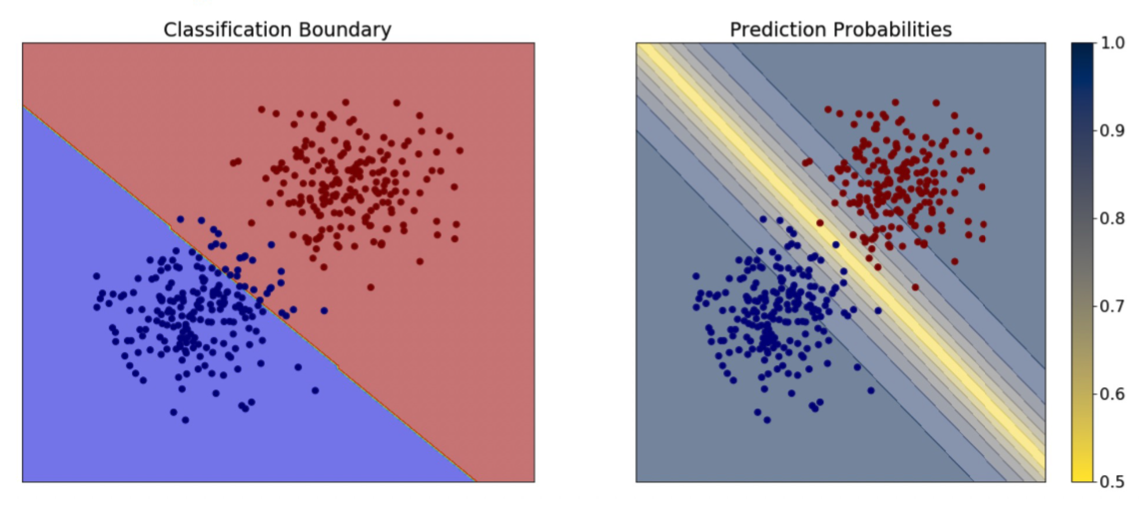
\includegraphics[width=\columnwidth]{asymmetric-cost.png}

\subsection{Abstention}

Another cost function could be used to decline to make a classification (action $D$):

$$C(y,a) = \begin{cases}
	\mathbb{I}_{y \neq a} & \text{if } a \in \{-1, +1\} \\
	c & \text{if } a = D
\end{cases}$$

\includegraphics[width=\columnwidth]{abstention.png}

\subsection{Uncertainty Sampling}

Labelling is often expensive since we need an expert to classify the samples. We want to minimize the actual number of labels that need to be hand classified. There is a simple strategy for this, always pick the sample that we are most uncertain about, by estimating $p(y \; | \; x)$, and then asking the expert to label this sample.